%
% Szakdolgozat minta az Eszterházy Károly Egyetem
% matematika illetve informatika szakos hallgatóinak.
%

\documentclass[
% opciók nélkül: egyoldalas nyomtatás, elektronikus verzió
% twoside, % kétoldalas nyomtatás
% tocnopagenum,% oldalszámozás a tartalomjegyzék után kezdődik
]{thesis-ekf}
\usepackage[T1]{fontenc}
\PassOptionsToPackage{defaults=hu-min}{magyar.ldf}
\usepackage[magyar]{babel}
\usepackage{mathtools,amssymb,amsthm,hyperref,listingsutf8,xcolor,caption,pdfpages}
\usepackage{subcaption}
\usepackage{float}
\lstset{
	inputencoding=utf8,
	language=C,
	basicstyle=\footnotesize,
	breaklines,
	captionpos=b,
	postbreak=\hbox{$\color{red}\hookrightarrow\ $},
	xleftmargin=1cm,
	xrightmargin=1cm,
	backgroundcolor=\color{gray!30},
	frame=tlbr,
	framesep=3pt,
	keywordstyle=\bfseries\color{green!40!black},
	commentstyle=\itshape\color{purple!40!black},
	identifierstyle=\color{blue},
	stringstyle=\color{brown},
	rulecolor=\color{black},
	showstringspaces=false
}

\captionsetup{compatibility=false}
\footnotestyle{rule=fourth}

\newtheorem{tetel}{Tétel}[chapter]
\theoremstyle{definition}
\newtheorem{definicio}[tetel]{Definíció}
\theoremstyle{remark}
\newtheorem{megjegyzes}[tetel]{Megjegyzés}

\begin{document}
\institute{Matematikai és Informatikai Intézet}
\title{Okos otthon hub és irányítóközpont}
\author{Lovász Ákos\\Programtervező informatikus BSc}
\supervisor{Dr. Tajti Tibor\\Egyetemi adjunktus}
\city{Eger}
\date{2021}
\maketitle
\tableofcontents


\chapter*{Bevezetés}
Tanulmányaim folyamán számos technológiával ismerkedtem meg, melyek mindegyike rengeteg
lehetőséget tárt fel előttem, viszont a szakmai gyakorlatom során kiemelkedően megragadta a fantáziámat az Andoid
fejlesztés és a hardverprogramozás összekapcsolása által kialakult rendszerek lehetősége.
\par
Az Android alkalmazások fejlesztése iránt mindig is érdeklődtem, egy-egy kisebb alkalmazást gyakorlásként
már készítettem ezt megelőzően, de komolyabban itt kezdtem vele foglalkozni, megismerkedni a vele járó
sajátosságokkal.
\par
Az ilyen jellegű eszközök kapcsolata és kommunikációja már korai gondolataimban is az okos otthonok felépítésére
emlékeztetett, ezért is gondoltam megfelelő táma választásnak.
\par
A döntést követő kutatás során szembetűnő hátránya volt az okos otthon rendszereknek, hogy a legtöbb ,,márkás''
megoldás elsősorban drága és csak felületes hozzáférést tesznek lehetővé, melyet teljes mértékben a rendszer
gyártója határoz meg. 
\par
Az alternatív, olcsóbb rendszerek bár nyíltabb hozzáállással próbálnak előnyt szerezni,
viszont sokszor erősen a technikai oldalába mélyednek, így egy átlagos felhasználónak bonyolultnak, 
nehezen kezelhetőnek tűnhetnek. Ezen felül gyakran futhatunk olyan problémába, hogy az általunk választott
rendszerben lévő hiányosságokat csak más gyártótól származó eszköz nyújtana megoldást, viszont különböző
gyártók eszközei nagyon ritkán kompatibilisek egymással.
\par
Ezeket az észrevételeket figyelembe véve egyértelműnek tűnt, hogy van lehetőség egy olyan rendszer kivitelezésére,
ami elsősorban olcsóbb, de ugyanakkor nem túlbonyolított, felhasználóbarát marad. Fontos a nyitottság, a bővíthetőség,
és a széleskörű kompatibilitás lehetősége, hogy a felhasználó biztos lehessen abban, hogy a jövőben felmerülő
hiányosságok egyszerűen pótolhatók.



\chapter{A rendszer alapjai}
A rendszer két fő komponensből áll. A kiszolgáló, mely egy Orange Pi Zero egykártyás számítógép, amin fut a Node-RED, egy olyan webes felületet biztosító szolgáltatás, mely grafikusan kezelhető komponensek összekapcsolásával teszi lehetővé a renszer működését befolyásolni, és a Mosquitto MQTT bróker, ami lehetővé teszi a Node-RED\cite{nodeRed} és az Androidos alkamazás közötti kommunikációt.

\section{A kiszolgáló hardver}
\begin{figure}
	\centering
	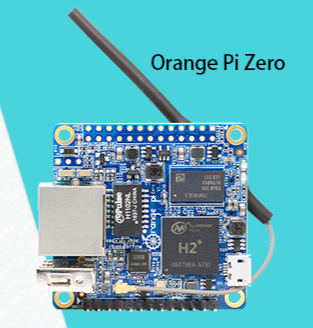
\includegraphics[width=0.5\textwidth]{images/OPIZero.png}
	\caption{Orange Pi Zero\cite{orange}, a Node-RED-hez és az MQTT brókerhez használt eszköz}
\end{figure}	
Az eszköz egy nyílt forráskódu egykártyás számítógép, amin Armbian\cite{armbian} (ARM processzor architektúrára specializált Debian) operációs renszer fut, 
de lehetőséget nyújt Ubuntu, vagy akár Android operációs rendszer telepítésére is. Ezen fut a Node-RED felület és a Mosquitto MQTT bróker, 
melyeket a helyi hálózaton bármely eszköz el tud érni, csupán az eszköz IP címét kell ismernie.

\section{Az Android alkalmazás}
Az Androidos alkalmazás célja a felhasználónak hozzáférést nyújtani az összes elérhető eszközhöz, 
azok állapotát megjeleníteni és felületet biztosítani azok irányítására, állapotuk megváltoztatására. 

A kiszolgálóval való kommunikációt az Eclipse nyílt forráskódú Paho\cite{paho} Androidos kliens oldali MQTT implementációját használatba véve valósítja meg az alkalmazás. 

A kommunikáció két irányú, azaz nem csak az alkalmazás tudja az okos eszközöket irányítani, 
hanem fogad üzeneteket a kiszolgálótól, így tud naprakész információt prezentálni az eszközök állapotáról a felhasználó számára.

A felület rugalmasságából adódóan az alkamazás nem kizárólag okos otthon kezelésére alkalmas, bármilyen MQTT protokoll alapú rendszeren való kommunikációra képes,
viszont miven a fejlesztés során az okos otthonok kezelése volt az elsődleges szempont, így erre a célra használva a legoptimálisabb a felhasználói élmény.

\section{Node-RED}
A Node-RED egy nyílt forráskódú, ,,flow'' alapú programozási eszköz az IBM Emerging Technologies\cite{ibmET} által fejlesztve az OpenJS Foundation\cite{openjs} részeként. 
Ez egy Node.js alapú fejlesztési eszköz, aminek a felületét egy böngészőn keresztül lehet elérni ahol ,,node''-okat elhelyezve a felületen  egy funkcióhálózatot létrehozva lehet úgymond programozni. 
Ez a funkcióhálózat egy ,,Deploy'' gomb hatására bekerül a futási környezetbe, így effektíve az eddigi viselkedést felülírva, változtatásainkat elmentve.

\section{MQTT}
Az MQTT (Message Queueing Telemetry Transport)\cite{mqtt} egy OASIS szabványú kommunikációs protokoll, 
melyet IoT (Internet of Things) eszközök kommunikációjához fejlesztettek ki. 
A protokoll alapja a ,,Publish/Subscribe'' alapú kommunikáció, azaz egy eszköznek lehetősége van egy adott ,,topic''-ra üzenetet továbbítani, 
vagy feliratkozni, azaz az adott ,,topic''-on beérkező üzeneteket megkapni. Ezek az üzenetek egy brókeren keresztül érik el céljukat, 
mivel a bróker tárolja hogy mely eszkör milyen témára iratkozott fel, ez alapján tudja a megfelelő klienseknek továbbítani a megfelelő üzenetet. 
Mivel az MQTT IoT eszközök kommunikációjához készült, így fejlesztése alatt különös figyelmet fordítottak az erőforrások megspórolásához, 
ezért ez a protokoll nagyon kevés erőforrást vesz igénybe, szinte bármilyen eszköz használatba tudja venni.

\section{Okos eszközök}
Okos eszköznek számít bármilyen berendezés, mely rendelkezik hálózati kommunikációra képes alkatrészekkel, 
ebben az esetben egy MQTT protokollt használatba vevő eszköz. Az MQTT protokoll rugalmasságából adódóan már a renszer tesztelése során is több eszköztípust 
vettem használatba, pédául Androidos tableteket, telefonokat és ESP D1 Mini mikrokontrollereket.



\chapter{Hardver}
\section{Orange Pi Zero}
Egy egykártyás számítógép az Orange Pi felhozatalából a Zero model, ami beépített WiFi modullal, Ethernet porttal, 
512MB RAM-al és egy 4 magos ARM processzorral ellátva tesztjeim alapján egy kisebb ház okos eszközeinek ellátására elegendő, 
viszont természetesen van lehetőség erősebb hardveren futtatni a kiszolgáló szolgáltatásokat. Ezek a szolgáltatások 
Linux és Windows operációs rendszert futtató hardverek bármelykén képesek futni, így lehetőségünk van akár 
régi, már nem használt androidos telefonon, vagy ellentétsen, csak erre a célra kitűzött szervergépet kialakítani. Természetesen 
a végletek között rengeteg lehetőségünk van igényeink szerint válatsztani kiszolgáló hardvert, például egy Orange Pi Zero, Raspberry Pi 4, vagy Seeed Odyssey.
Az Orange Pi Zero-ra esett a választásom alacsony ára mellett nyújtott lehetőségei tárháza miatt.
\section{Okos eszközök}
\subsection{ESP 8266}
Okos eszköz fejlesztéséra egy rendkívül olcsó lehetőség az ESP D1 Mini mikrokontroller, ami Arduino nyelven
programozható, WiFi moduljának és a hivatalos Arduino MQTT könyvtárnak köszönhetően viszonylag egyszerűen okos otthon eszközzé lehet alakítani.
\subsection{Androidos eszköz}
Mivel az Androidos alkamazások bizonyos könyvtárai és fejlesztői eszközei az alkalmazott Android verziótól függnek, így az alkalmazás fejlesztése során
kitűzött minimum Android verziót el kell érnie a használni kívánt eszköznek. Ebben az esetben a minimum támogatott Android verzió a Marshmallow, azaz Android 6.0.
Ez a legrégebbi Android megjelenés amit bevett szokásként támogatnak a modern alkamazások, ennél korábbi verziót támogatni nehézkes, általában nem éri meg, mivel
a felhasználók kevesebb mint 1\%-a használ olyan eszközt, ami 6.0-nál régebbi Androidot futtat.
\subsection{Egyéb eszközök}
Minden olyan okos eszköz integrálható a rendszerbe, amely képes MQTT protokollon keresztül kommunikálni egy helyi hálózaton.



\chapter{Szoftver}
A teljes rendszer olyan módon van felépítve, hogy a szerver oldali programoktól elvárt, hogy állandó futás mellett lehetőséget 
nyújtsanak bővítésre, konfigurációra és változtatásokra. 
\section{PM2}
Az állandó futást a PM2\cite{pm2} nevű folyamatvezető program biztosítja, akár egy váratlan újraindítás vagy áramkimaradást követően az operációs rendszer indulásával ezek a programok is indulnak, megfelelő konfigurációval.

\begin{figure}[h]
	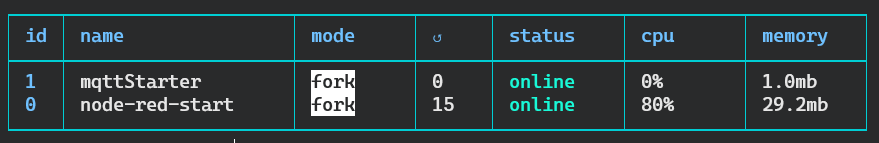
\includegraphics[width=1\textwidth]{images/pm2.png}
	\caption{PM2\cite{pm2} a kiszolgálók automatikus indítására használt eszköz}
\end{figure}

Ez a terminálban futtatható Node.JS eszköz egyszerűen telepíthető NPM vagy Yarn csomagkezelőkkel, és azonnal használatba vehető.
Lehetőséget nyújt nem csak Node.JS alkalmazások futtatására, de egyéb futtatható fájlok kezelésére is, például shell scriptek futtatására.

\section{Node-Red}
\subsection{Flow}
A Node-Red rendszerben csomópontok elhelyezésével és azok összekötésével lehet egy folyamatábrára hasonlító szerkezetet kiépíteni, 
ami a program viselkedését befolyásolja. Minden csomópont egy funkciót lát el, ehez mérten van a csomópontnak 
egy vagy több bemeneti és/vagy egy vagy több kimeneti pontja, amin keresztül kommunikál a többi csomóponttal.

Egy ,,flow'' a Node-Red felületén a benne lévő csomópontok és azok kapcsolatát foglalja magában. 
Minden flow reprezentálhat egy házban egy-egy szobát, nagyobb rendszereknél pédául egy-egy épületet, vagy több emeletes épületekben egy-egy emeletet.
Ez felhasználható rendszerezési, kategorizálási vagy szerepköri felosztásra is, teljes mértékben a felhasználótól függ.

\begin{figure}[h]
	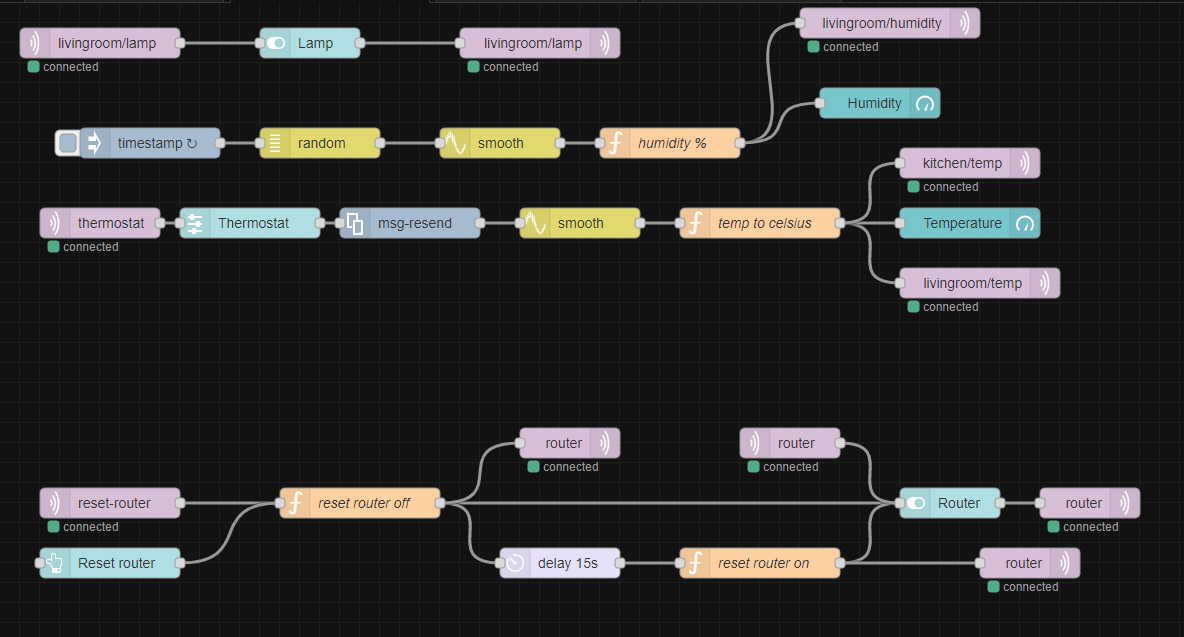
\includegraphics[width=1\textwidth]{images/flow.png}
	\caption{Minta ház nappali flow}
	\caption{Egy minta ház kiépítésében a nappaliban található eszközök irányítása}
\end{figure}

Az MQTT csomópontok belső konfigurációja csupán két dolgot vár el felhelyezése során: az MQTT topic, amire az adott csomópont feliratkozik, és az MQTT bróker címe. A bróker címét minden MQTT csomópont megosztja, így a kiszolgáló címének változásakor
elég egy helyen megváltoztatni a címet, az összes csomópont megkapja az új címet és újra tud csatlakozni.

Implementáltam minden szobába egy okos lámpát, hőmérőt és páratartalom mérőt. Ezen felül a nappaliban és a hálószobában vagy egy-egy termosztát, melyeket függetlenül irányíthatunk. Mivel ez a minta ház csak szimuláció, így a szemléltetés érdekében
a hőmérsékletváltozást egy időintervallum alatt fokozatosan változtatom a termosztát állítást követően, így reprezentálva a való világban a ház fokozatos felfűtését/lehűtését. Szintén szemléltetési céllal a páratartalom mérők
véletlenszerű értékeket vesznek fel, mivel egy bemutató példa házban nem szükséges a valóságnak megfelelő értékeket szimulálni, a rendszer szemléltetése a lényeg.

Az okos lámpa egy egyszerű kapcsolóként jelenik meg a bemutató házban, ez természetesen egy okos kapcsolóval ellátott lámpát reprezentál, melyet irányíthatunk az Androidos alkalmazásból, vagy a webes felületről.

Ezen felül felhelyeztem egy internet router újraindító gombot, ezzel adva példát egy egygombos funkió ellátására, mivel egyszerűbb egy újraindítás gombot megnyomni, 
mint kapcsolóként kezelni és a felhasználóra bízni, hogy ne kapcsolja vissza idő előtt a router-t, így megelőzve az esetleges 
késés által előidézett időkimaradás eltörlését, mivel az MQTT sorban küldi az üzeneteket, ha a rendszer lelassul egy pillanatra, 
lehet, hogy két üzenet, amit a felhasználó egymástól eltérő időpintban küldött el, mégis egyszerre érkezik a kiszolgálóhoz.

Ez a webes szerkesztőfelületet a helyi hálózaton a kiszolgáló eszköz IP címén, a konfigurációban megadott portszámon (alapbeállítás szerint 1880) lehet elértni.
Az itt végzett változtatások csak akkor kerülnek a futási környezetbe, ha a ,,Deploy'' feliratú gombot megnyomjuk, különben minden változtatás
csak a felületen történik, átmenetileg van mentve, hogy közben a szolgáltatás az előző verzióval tovább tudjon futni, így
állandó elérést és irányítást biztosítva a már felcsatlakozott okos eszközök számára.

\subsection{Dashboard}
A Node-Red lehetőséget nyújt egyéb csomópontok telepítésére, melyeket felhasználók vagy egyéb entitások fejlesztettek. 
Egy ilyen csomópont kollekció a Node-Red Dashboard\cite{dashboard}, mely által lehet készíteni egy webes felületet, amin keresztül lehet szemléltetni, irányítani a rendszer elemeit. 
\begin{figure}[h]
	\centering
	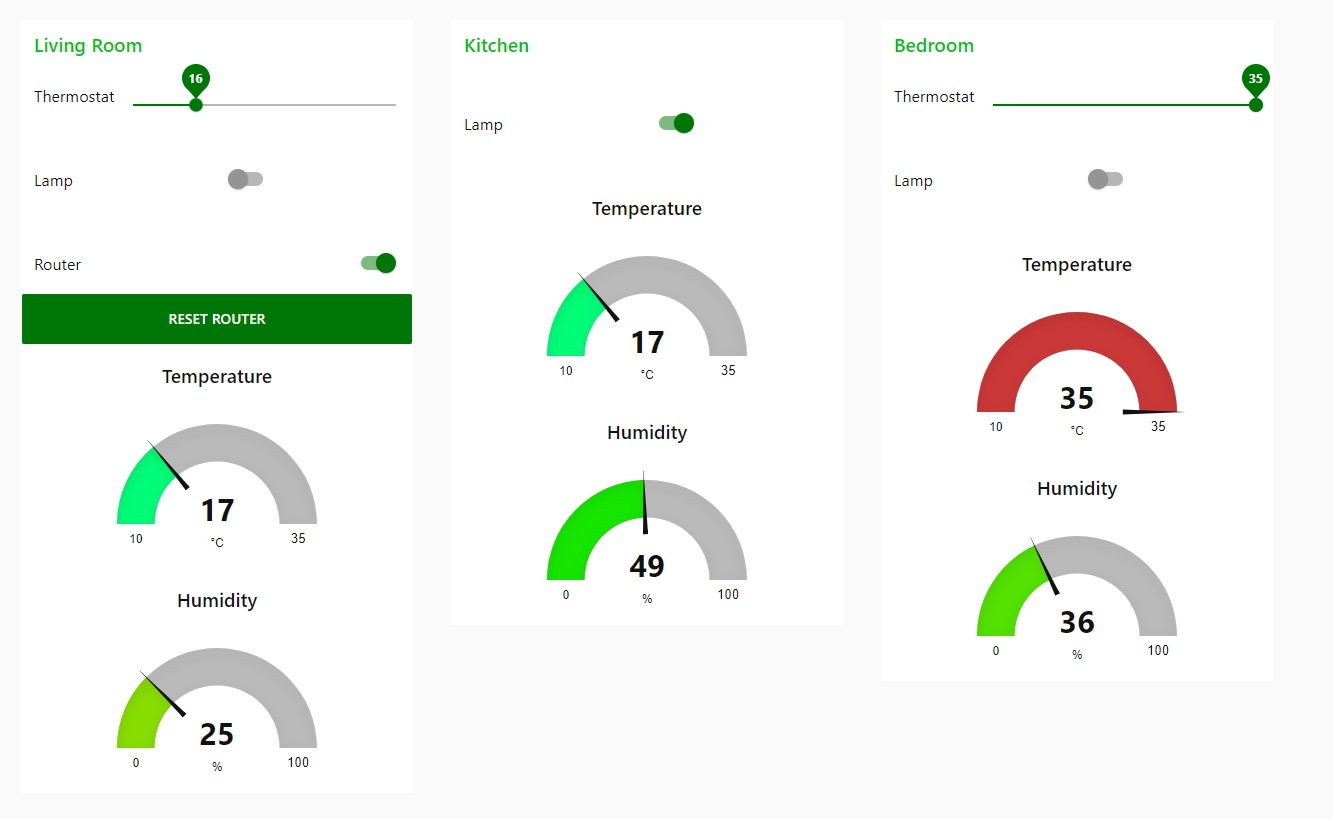
\includegraphics[width=0.8\textwidth]{images/dashboard.jpg}
	\caption{A Node-Red Dashboard\cite{dashboard}, szobákra bontva, példa eszközökkel ellátva}
\end{figure}


Ez nem olyan rugalmas, mint az Android alkalmazás, mivel minden
elemet kézzel kell felvenni a felületre, majd minden konfigurációját és interakcióját a flow szerkesztőben kell kézileg megadni, minden elemet külön fel kell programozni.

\section{MQTT}
\subsection{Broker}
MQTT brókernek az Eclipse Mosquitto\cite{mosquitto}-t választottam, mivel egy jól ismert alapítvány által fejlesztett, teljesen nyílt forráskódú multi-platform projekt,
melyben különös figyelmet fordítottak az erőforrásokkal való spórolásra, így egykártyás számítógépeken való alkamazását megkönnyítve. 

Szintén előnyt jelentett választásom során a jó minőségű dokumentáció, mely alapján
viszonylag zökkenőmentes volt a telepítés és a konfiguálás.
\subsection{Konfigurálás}
Mivel a konfigurációs fájlban meg kell adni a brókernek, hogy mely címen fog csatlakozási kérelmeket és üzeneteket kapni,
készítettem egy olyan shell scriptet, mely minden indításnál egy új, naprakész konfigurációs fájlt készít a bróker indítása előtt.

\lstset{language=bash}  
\begin{lstlisting}[frame=single]
echo -n "listener 1883 " > mqtt.conf; ip -4 addr show eth0 | grep -oP '(?<=inet\s)\d+(\.\d+){3}' >> mqtt.conf echo $"allow_anonymous true" >> mqtt.conf
\end{lstlisting}

Ez a shell script generál egy olyan konfigurációs fájlt, ami a következőket állítja be:
\begin{itemize}
	\item 1883-as porton várja az üzeneteket
	\item Lekérdezi a kiszolgáló számítógép IPv4 címét, amit egy regex szűrőn keresztül formázom megfelelő módon és a portszám után illesztem be, előírás szerint.
	\item Engedélyezi az anoním kapcsolatokat. Mivel ez a rendszer egy helyi hálózatra van tervezve, nem jelent biztonsági kockázatot az autentikáció nélküli kapcsolat, ezt kiváltja az MQTT ID rendszer.
\end{itemize}

\section{Android}
\subsection{Activity}
Az Android ,,aktivitásokra'' bontja a kódot, melyek a hozzájuk tartozó ,,töredékek'' alappilléreként szolgál.
Fő célja az aktivitásokra bontásnak az erőforrások megspórolása, minden aktivitás egy specifikus feladatkört lát el, 
miközben a másik aktivitások a háttérben leállnak, amíg nem lépnek újra használatba. Az én esetemben egy fő aktivitás
látja el az alapvető feladatait az applikációmnak, mivel ennek a fő aktivitásnak a kiszolgálóval való kapcsolattartás és
a felhasználói adatok tárolása, így több aktivitásra bontani ezt csak feleslegesen bonyolítana mind a program logikáján,
mind az átláthatóságán.

Az Android rendszer alapjáraton 4 fő ,,szálat'' különböztet meg:
\subsubsection{Main Thread}
A fő szál. Ez az alkalmazás indításakor az operációs rendszer által nyitott szál, mely felelős az események kezeléséért, felhasználói felület megrajzolásáért és egyéb elemek létrehozásáért.
	
\subsubsection{Ui Thread}
A felhasználói felületi szál, ami felelős a felhasználóval való kapcsolat fenntartásáért 
és a felületi eseménykezelésért mint például egy gomblenyomás. Fontos, 
hogy a UI szálat sosem szabad megakasztani hosszú folyamatokkal, 
például hálózati csatlakozás indításával, mivel ilyenkor a felület teljes egészében leáll, 
a felhasználó felé nem reszponzív, nem tud semmilyen eseményt kezelni 
amíg a folyamat ami megakasztotta a szálat be nem fejeződik.
	
\subsubsection{Worker Thread}
Az egyéb többszálas folyamatokat kezelő szál. Ez a szál nyújt megoldást a UI szál megakasztására,
ezt kell használni hosszabb, nem azonnal ellátható események kezelésére. Felmerül használata során viszon az a
probléma, hogy a felhasználói felületet csakis a UI szálról lehet frissíteni. 
	
\subsubsection{Binder Thread}
A kötött szolgáltatások távolról meghívható metódusokat tartalmaznak. Ha a végrehajtott metódusra történő felhívás ugyanabban a folyamatban van, amelyben a kötött szolgáltatás fut, a metódus a hívószalagban hajtódik végre. Ha azonban a hívás egy másik folyamatból származik, akkor a metódus egy olyan szálban kerül végrehajtásra, amelyet a rendszer ugyanabban a folyamatban tart, mint az meghívó.

\subsection{Fragmentek}
A fragment az része az alkalmazás felhasználói felületének, ami saját felosztását definiálja és kezeli. Saját életciklussal
rendelkezik, viszont egyedülálló elemként nem használhatóak, mindig kell lennie egy tulajdonosának, ami lehet egy másik
fragment vagy activity. Ehez a tulajdonoshoz kötve jelenhet meg egy fragment felülete hozzá csatolva vagy részévé válva.

A fragmentek célja hogy egy activityn belül külön választott felhasználói felületet prezentálhassunk, egymástól független
elemekre bontva, így megkönnyítve a felhasználói felület felépítésének procedúráját és az erőforrások megtakarítását.

A fragmentek ideális használati köre egy activityn belüli navigációs elemek által elérni kívánt felületek prezentációja. Mivel egy fragment életciklusa akkor ér véget, amikor a felhasználó egy másik fragmentre váltással felülírja azt, hosszútávú
adattárolásra nem alkalmas, bár erre is vannak beépített megoldások, például a fragmentet tartalmazó activiy szintjén tárolni
az adatokat, vagy a fragmentek belső ,,instance bundle'' változójával kezelni, bár az utóbbi típusmegközései miatt igencsak
korlátozó módszer, de több módszer kombinálása sem kizárt, így mindent olyan módon lehet kezelni, ahogyan az adott esetben optimális.
\subsection{Felhasználói felület}
Az alkalmazásom felhasználói felülete 3 fő fragmentből áll: Home, Settings és Help. A Home fragment a fő interakciós felülete
az alkalmazásnak, itt tölti a felhasználó az ideje nagy részét, itt éri el és irányíthatja a hálózaton található okos eszközöket.

A Settings fragment a kiszolgáló címének megadására, felhasználói profil kiválasztására és a kapcsolat létesítésére
szolgál.

A Help fragment felhasználási segítséget nyújt a felhasználó számára, ha nem biztos az alkalmazás működésének rendjében,
ezen leírás alapján tud tájékozódni a rendeltetésszerű felhasználásról.
\subsubsection{Home}
A Home fragment szolgál az eszközök kezelésére, irányítására, adatok prezentálására.
A felület jobb alsó sarkában található ,,Floating Action Button'', vagy FAB megnyomására a felhasználó feliratkozgat egy MQTT
topicra, majd kiválaszthatja a létrehozandó kártya interakciós típusát. 

Ha sikeresen feliratkozik egy topicra, a felületen létrejön
egy ,,kártya'' a kiválasztott interakciós típussal, például egy csúszkával, gombbal vagy kapcsolóval. Ezt követően a felhasználó a
kártyán keresztül tudja kezelni az adott topicot használó okos eszközöket. 

Ha a felhasnáló el szeretné távolítani a kártyát a felületről,
egy hosszú érintéssel a kártya bármely részére előidéz egy ,,Unsubscribe'' kontextusi gombot, melyel törölheti a kártyát a felületről.

\begin{figure}[H]
	\centering
	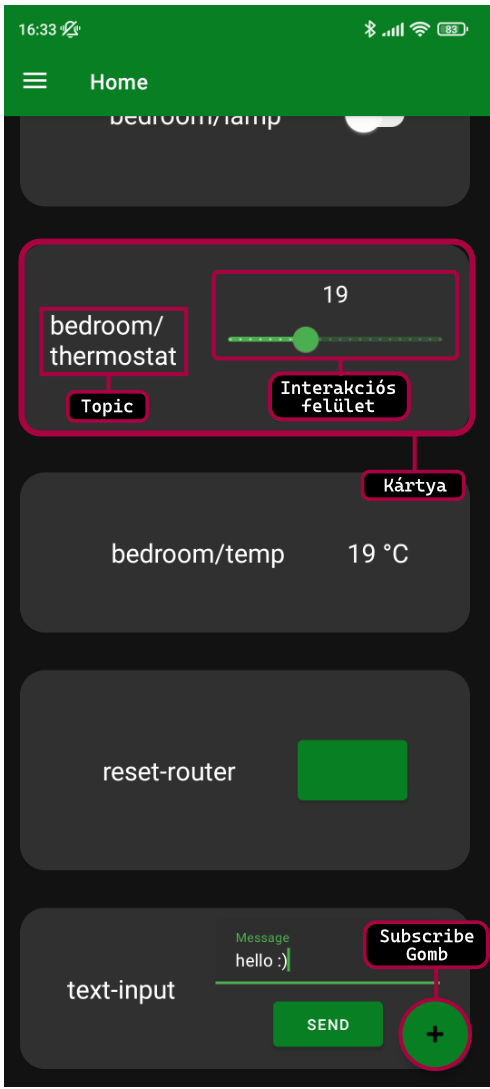
\includegraphics[width=0.5\linewidth]{images/home_anatomy.png}
	\caption{A Home fragment elrendezése és elemei}
	\label{fig_home_anatomy}
\end{figure}
	
\subsubsection{Settings}
A Settings fragment a kiszzolgálóhoz való csatlakozásra és a felhasználói profil beállítására szolgál.

A felületen található két beviteli mező. Az elsőbe a felhasználói profil elnevezését, a másodikba a kiszolgáló címét
kell megadni, majd a ,,Connect'' gomb megnyomására az alkamazás kapcsolatot létesít a kiszolgálóval és ellenőrzi, hogy
létezik-e már a megadott néven felhasználói profil. Ha már létezik, az alkamazáson belüli tárba betölti az elmentett adatokat,
viszont ha nincs, létrehozza azt.

A ,,Delete Profile'' gomb egy új ablakban, legördülő menüből kiválasztható profilok listájából törli azt, amelyket a
felhasználó kiválaszt.
\begin{figure}[H]
	\centering
	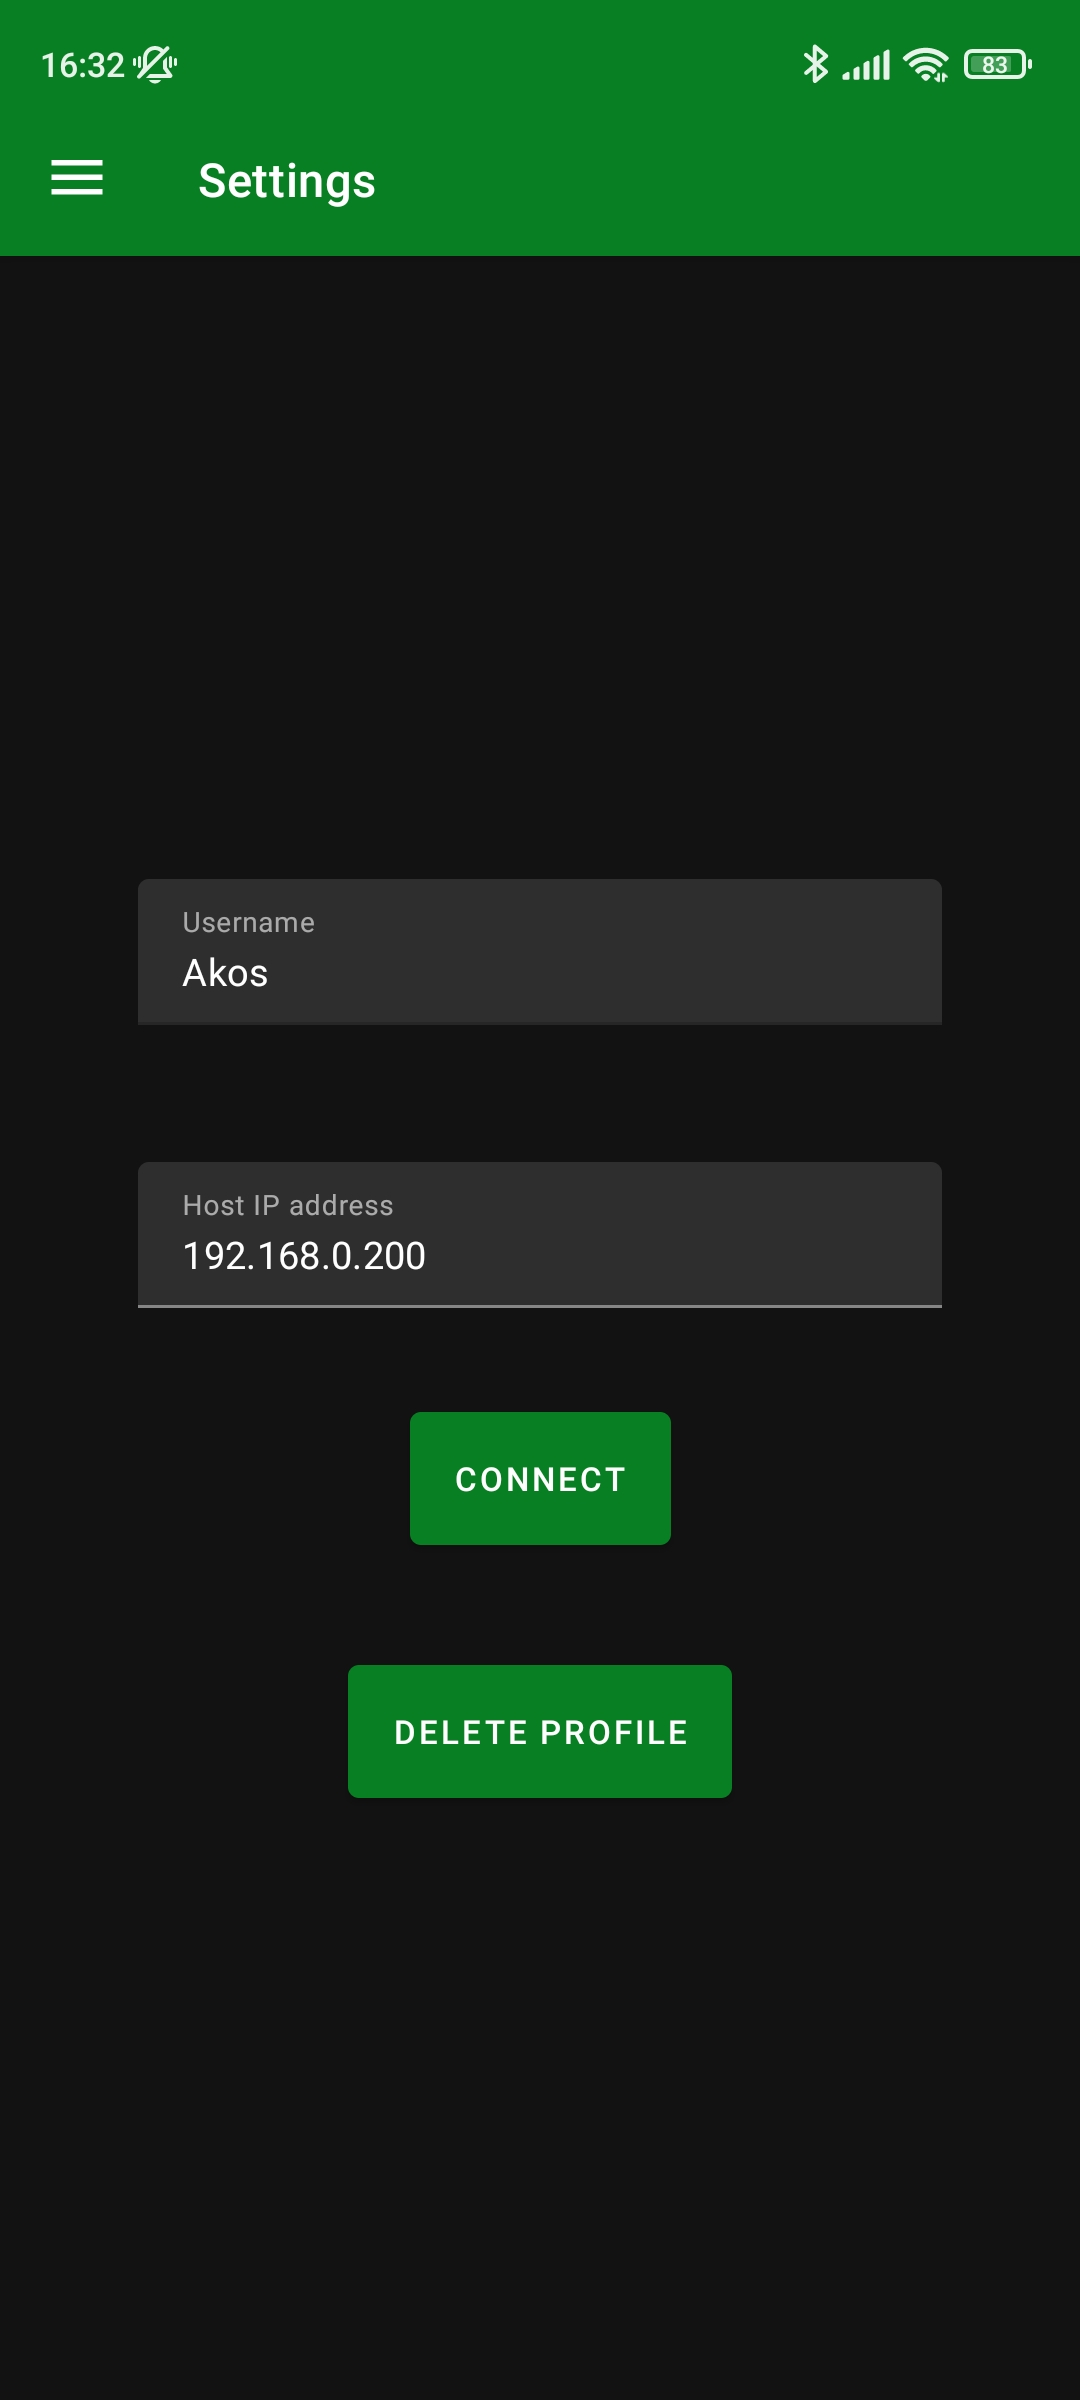
\includegraphics[width=0.5\linewidth]{images/connect.jpg}
	\caption{A beállításokat tartalmazó fragment}
\end{figure}

Az itt megadott értékeket az alkalmazás eltárolja, így a következő indításkor ezek a mezők már az előző használatkor
alkalmazott értékekkel kitöltve jelennek meg, így megkönnyítve felgyorsítva az alkalmazás használatát.

\subsubsection{Help}
A help fragment tartalmazza a felhasználói útmutatót. Itt lehet tájékozódni az alkalmazás rendeltetésszerű használatáról,
a funkciók céljáról, használatáról és az esetleges problémák megelőzéséről, kijavításáról.

A help fragment szintén kártyákra osztja a felületet a könnyű és gyors átláthatóság érdekében és a
konzisztencia fenntartásáért.

\subsection{Kapcsolat}
Az MQTT kapcsolatot Android oldalon szintén az Eclipse Foundation megoldását használom, a paho\cite{paho} nevű,
nyílt forráskódú MQTT kliens Android implementációját, a Geradle rendszeren keresztül összeállított,
Maven repositoryból leöltött forrás csomagját importálva.

A kapcsolat 60 másodperces időtúllépést elérve felbontódik, ha nem kap választ a kiszolgáló az életben tartó
jelre. Ezért a kapcsolat létrehozása pillanatában a kliens entitását eltárolom egy activity szintű változóban,
így a kapcsolat addig él, amíg a felhasználó használja az alkamazást, vagy nem zárja be több mint 1 percre.

\lstset{language=Java}  
\begin{lstlisting}[frame=single]
MqttAndroidClient client = new MqttAndroidClient(this.getApplicationContext(),
"tcp://" + mqttAddress + ":1883", clientId);

client.connect(null, new IMqttActionListener() {
	@Override
	public void onSuccess(IMqttToken asyncActionToken) {
		mqttClient[0] = client;
	}

	@Override
	public void onFailure(IMqttToken asyncActionToken, Throwable exception) {
		Toast toast = Toast.makeText(getApplicationContext(),
				"Failed to connect to " + mqttAddress, Toast.LENGTH_SHORT);
		toast.show();
	}
});
\end{lstlisting}

Ez a kapcsolat aszinkron módon jön létre, így nem kell megállítani a felhasználót, amíg nem jön létre a
kapcsolat, vagy hibát eredményez a csatlakozás, például hibás címet adott meg a felhasználó vagy
a kiszolgáló nem fut.

\subsection{Kártyák}
A jelenlegi verzióban 6 típusú kártya használatára van lehetőség, de ez a jövőben egyszerűen bővíthető:
\begin{itemize}
	\item Text: Szimpla szöveges feliratot prezentál, felhasználható pédául hőmérő értékének kijelzésére.
	\item Button: Egy gombot tartalmaz, ami az adott topic-ra egy "1"-es üzenetet küld, amit a kiszolgáló
	dolgoz fel.
	\item Checkbox: Egy jelölőnégyzet, mely "on" és "off" üzenetet küld a kiszolgálónak állapota szerint.
	Lehet használni sokoldalú állapotjelzőnek vagy kapcsolónak.
	\item Swithc: Egy kapcsoló, mely szintén "on" és "off" üzenetet küld a kiszolgálónak állapota szerint,
	így logikusan alkalmazható például okos lámpa kapcsolójaként.
	\item Input: Egy beviteli mezőt tartalmaz, amibe tetszőleges szöveget vagy számot írhat a felhasználó,
	majd az alatta lévő gomb érintésével elküldi a tartalmát az adott topic-ra. Használható például LED-es
	tábla feliratának módosítására.
	\item Slider: Egy csúszka, melynek minimum és maximum értékeit a felhasználó határozza meg, az ez
	által nyújtott sokoldalúságából eredendően lehet használni például termosztát beállítására, vagy
	okos lámpa fényerejének módosítására.
\end{itemize}

Egy kártya felépítése a korábban látott ábra szerint (\ref{fig_home_anatomy}) két félre bontódik.
Bal oldalán található a topic felirata, amelyre az adott kártya feliratkozott. 

A jobb oldalán található
a felhasználó által választott interakciós felület, melyen keresztül tud kommunikálni az alkalmazás a
kiszolgálóval az adott topic-on. 

Minden kártya egymástól teljesen független, így például több kártya ugyan
arra a topicra képes feliratkozni, nem okoz problémát, minden kártya feldolgozza a rá vonatkozó,
azaz a topicra érkező üzeneteket.

Egy törönni kívánt kártyát a hosszú érintésével előidézhető ,,Unsubscribe'' gomb megnyomásával tudunk
eltávolítani a felületről. Ez nem csak vizuálisan szűnteti meg az adott kártyát, de a topicról is
leiratkozik, amit eddig használt, így azt a minimális erőforrást is felszabadítva amit elfoglalt. 

Mielőtt egy kártya sikeres feliratkozás eredményeként létrejön, több adatfeldolgozási lépést kell megtenni. 
Vegyünk példának egy kapcsoló típusú kártyát:


\lstset{language=Java}  
\begin{lstlisting}[frame=single]
private void createCard(LinearLayout layout, List<String> savedCardData, int type) {
    ViewGroup mqttCard = (ViewGroup) this.getLayoutInflater().inflate(type, null);
    TextView topicDisplay = (TextView) mqttCard.findViewById(R.id.text_topicDisplay);
    registerForContextMenu(mqttCard);
    topicDisplay.setText(savedCardData.get(0));
\end{lstlisting}

A kártya létrehozó metódusa megkapja paraméterként a Home fragment alapelrendezését, amiben majd el kell
helyeznie az új kártyát, egy listát, ami tartalmazza a profilban tárolt kártyák adatát, így ha már
volt a profilban mentett adat, azt visszaállítja a program, nem kell újból azokat megadni, és végül
megkapja a kártya típusát, mely alapján kiválasztja a program, hogy milyen interakciós felületű kártyát
hozzon létre.

Ezt követően inicializálja a kártya struktúra alapját, a topic kijelző szövegét, és elkezdi a kártyatípus ellenőrzését.

\lstset{language=Java}  
\begin{lstlisting}[frame=single]
switch (type) {
	case R.layout.mqtt_card_switch:
                SwitchMaterial switch_data = (SwitchMaterial) mqttCard.findViewById(R.id.switch_data);

                if (!savedCardData.get(2).equals("null")) {
                    switch_data.setChecked(savedCardData.get(2).equals("on"));
                }
                switch_data.setOnClickListener(view -> {
                    String message = switch_data.isChecked() ? "on" : "off";
                    publishMessage(((MainActivity) getActivity()).getClient(), savedCardData.get(0), message);
                });
                layout.addView(mqttCard);
                break;
\end{lstlisting}

Miután a kártyatípus eldöntésre került, inicializálja a kártya létrehozásához szükséges változókat, majd ellenőrzi, hogy volt-e már az adott topicon ilyen típusú kártya mentve.
Ha volt mentett adat az adott kártyáról, azt állítja be kezdőértéknek
(ebben az esetben hogy milyen állapotban volt utoljára a kapcsoló).

Ezt követően létrejön az interakciós felület ,,figyelője'', mely megadja, hogy az adott felület használata
milyen módon reagáljon, ebben az esetben a kapcsoló állapotváltozása küld egy "on" vagy "off" üzenetet a
kiszolgáló számára, állásától függően.

Végül a kártya felkerül a felhasználói felületre.

\subsection{Kommunikáció}
kártyák, connect, disconnect, reconnect, background task
\subsection{Adattárolás, Profilok}
A kártyaadatok profilonkénti tárolása egy szöveges fájba való kiírással oldottam meg, olyan formátumban, hogy a fájl
neve a felhasználói profil megadott neve, a tartalma pedig minden kártya amit a felhasználó létrehozott, a következő
formában felbontva: Topic:Kártytípus:Tárolt adat.

Minden kiírás esetén ellenőrzöm, hogy már szerepel-e a fájlban a jelenleg mentésre kijelölt kártya, így elkerülve
felesleges kiíratási folyamatokat, ha már létezik, mivel ebben az esetben felesleges lenne kitörölni és újra kiírni.

Ez az ellenőrzés viszont csak a kártya topicra és típusra vonatkozik, mivel a tárolt adat folyamatosan változik.
Az ellenőrzés során megkeresem az összes olyan elmentett kártyát, ami ugyanazt a topicot és kártyatípust tartalmazza,
majd csak azt a sort írom felül a friss adatokkal, így nem kell a teljes fájlt újraírni csak egy sor módosításáért.

Friss profiloknál, mivel egy üres fájl jön létre, a kereső algoritmus hibát dobna, mivel nem tud üres sorokban
keresni, ezért erre az esetre egy külön elágazást implementáltam, ami szimplán kiírja a menteni kívánt kártya adatait,
mivel ebben az esetben biztosak lehetünk abban, hogy még nem tartalmazza a fájl ezt a kártyát, ezért átugorhatjuk az
ellenőrzést.


\lstset{language=Java}  
\begin{lstlisting}[frame=single]
public void addCardDataToPersistentStorage(String topic, String cardType, String cardData) {
	boolean found = false;
	int i = 0;
	if (cardDataStore.size() == 0) {
		this.cardDataStore.add(topic + ":" + cardType + ":" + cardData);
	}
	do {
		String[] part = this.cardDataStore.get(i).split(":", 0);
		if ((part[0] + ":" + part[1]).equals(topic + ":" + cardType)) {
			this.cardDataStore.set(i, topic + ":" + cardType + ":" + cardData);
			found = true;
		}
		i++;
	}
	while (!found && i < cardDataStore.size());

	if (!found) {
		this.cardDataStore.add(topic + ":" + cardType + ":" + cardData);
	}

	writeToFile(this.username + ".txt", this.cardDataStore);
}
\end{lstlisting}

A kártyák adatain kívül az alkalmazás tárolja az utoljára használt felhasználónevet és a kiszolgáló címét.
Ezt az Android sajátos ,,SharedPrefrence'' API eszközeivel tárolom, ami kulcs-érték párokat tárol, melyeket csak az
alkalmazáson belül lehet elérni.
Mivel ez a rendszer kis mennyiségű adatok tárolására célzott eszköz, így a kártyák adatainak tárolására nem lenne
alkalmas, viszont a felhasználónév és kiszolgáló címének tárolását beolvasztani a kártyaadat tárolására szolgáló
fájlba rendezetlen és bonyolultnak tűnt, ezért választottam szét a két tárolási módot.

A profilok törlésére a Settings fragmenten található ,,Delete Profile'' gomb megnyomásával van lehetőség,
ami kilistázza az összes profil fájl címét egy legördülő menüben.

\section{Tesztelés}
nem teszteltem :) bíztam benne hogy jólesz és jézusra bíztam az app stabilitását


\chapter{A renszer működése}
Itt írom le a kész rendszer működését, 
\section{Első indítás}
hátugye nem minden létezik first start
\subsection{Szerver}
mostly preconfigured de a flow lehet kell noderedbe meg mqtt config idk, meg ezeket telepíteni
\subsection{Android}
alkalmazást telepíteni, először nincs user de onnan minden magától megy
ha létezett a username akkor parsolja az adatot runtime-ba és onnan tovább szétszedi és kártyákat csinál

\section{Telefon csatlakoztatása kiszolgálóhoz}
ip, connect. ez async mqtt, ezt letárolom egy gettable mqttclinet változóban. persistent connection
timeout, message retention
\section{Okos eszközök kezelése az alkalmazásban}
sub to topics, makes cards
\subsection{Feliratkozás, Kártyarendszer}
dinamikus scrollview, mident tárol, kapott adatokat lebontja,
\section{Okos eszközök kezelése a webes felületen}
node-red ui, több vele a szarakodás mint androidon so nem előnyös, része az üzemeltetésnek


\chapter{Továbbfejlesztési lehetőségek}
user auth: bár mqtt-nél nincs sok értlme, maybe parentala controls
cloud service for out of home control
andoid auto-looks for the broker, this might be expensive and hard


\chapter*{Köszönetnyilvánítás}
\par
Köszönöm a vscode-nak hogy van,
\par
Köszönöm magyarországnak hogy jobban teljesít
\par
Köszönöm a covidnak, hogy átmentem nummatból
\par
Köszönöm anyádnak
\par
Köszönöm faszkivannak hogy nézte a streameket
\par
Köszönöm martinnak hogy helyettem is ivott, így én józanul tudtam dolgozni

\begin{thebibliography}{2}
\bibitem{nodeRed}Node Red forrás,
\\\texttt{\url{https://nodered.org}}

\bibitem{dashboard}Node Red Dashboard forrás,
\\\texttt{\url{https://flows.nodered.org/node/node-red-dashboard}}

\bibitem{orange}Orange Pi forrás,
\\\texttt{\url{http://www.orangepi.org/}}

\bibitem{mqtt}MQTT protokol forrás,
\\\texttt{\url{https://mqtt.org}}

\bibitem{mosquitto}Mosquitto bróker forrás,
\\\texttt{\url{https://mosquitto.org}}

\bibitem{paho}Paho Android MQTT implementáció,
\\\texttt{\url{https://www.eclipse.org/paho/index.php}}

\bibitem{material}Material design forrás
\\\texttt{\url{https://material.io/components/}}

\bibitem{android}Android fejlesztői dokumentáció
\\\texttt{\url{https://developer.android.com/guide}}

\bibitem{armbian}Armbian operációs rendszer
\\\texttt{\url{https://www.armbian.com/}}

\bibitem{iot}IoT based Smart Environment Using Node-Red and MQTT
\\\texttt{Deepthi, B. \& Kolluru, Venkata Ratnam \& Varghese, George \& Narne, Rajendraparasad \& Srimannarayana, Nerella. (2020). IoT based Smart Environment Using Node-Red and MQTT. Journal of Advanced Research in Dynamical and Control Systems. 12. 10.5373/JARDCS/V12I5/20201684.}
\\\texttt{\url{https://www.researchgate.net/publication/342327250_IoT_based_Smart_Environment_Using_Node-Red_and_MQTT}}
	
\bibitem{android refrences book}Android\texttrademark Notes for Professionals book
\\\texttt{\url{https://books.goalkicker.com/AndroidBook/}}

\bibitem{ibmET}IMB Emerging Technologies
\\\texttt{\url{https://emerging-technology.co.uk/}}

\bibitem{openjs}OpenJS Foundation
\\\texttt{\url{https://openjsf.org/}}

\bibitem{pm2}PM2 Process Manager
\\\texttt{\url{https://pm2.keymetrics.io/}}

\end{thebibliography}
%\includepdf{nyilatkozat.pdf}
\end{document}